\chapter{Results and Evaluation Framework}
\label{ch:results}

\section{Evaluation Protocol}

This chapter reports the executed evaluation framework and quantitative results. Training for each configuration uses fixed training schedules and consistent checkpoint intervals. Evaluation is performed under matched testing conditions across all compared methods, so the reported rankings are directly comparable.

\section{Evaluation Metrics}

We evaluate sinogram recovery quality using three complementary metrics that are widely adopted in image reconstruction studies~\cite{wang2004image}.

\subsection{Peak Signal-to-Noise Ratio (PSNR)}

PSNR measures the pixel-wise accuracy of the reconstructed sinogram relative to the ground truth:
\begin{equation}
\text{PSNR} = 10 \log_{10}\left(\frac{\text{MAX}^2}{\text{MSE}}\right)
\end{equation}
where MAX is the maximum possible pixel value and MSE is the mean squared error.

\subsection{Structural Similarity Index (SSIM)}

SSIM~\cite{wang2004image} evaluates perceptual similarity by comparing local structures:
\begin{equation}
\text{SSIM}(x, y) = \frac{(2\mu_x\mu_y + C_1)(2\sigma_{xy} + C_2)}{(\mu_x^2 + \mu_y^2 + C_1)(\sigma_x^2 + \sigma_y^2 + C_2)}
\end{equation}
where $\mu$, $\sigma$, and $\sigma_{xy}$ represent local means, variances, and covariance. SSIM ranges from 0 to 1, with 1 indicating perfect structural similarity.

\subsection{Mean Absolute Error (MAE)}

MAE provides a direct measure of average prediction error:
\begin{equation}
\text{MAE} = \frac{1}{N}\sum_{i=1}^{N}|x_i - \hat{x}_i|
\end{equation}
This metric provides a direct error measure in projection (sinogram) space. Clinical Hounsfield unit accuracy is assessed in reconstruction space rather than directly from sinograms.

\section{Baseline Method Comparisons}

We completed a baseline evaluation at a fixed operating point ($k_c=320$) for three learned methods (U-Net inpainting, Cold Diffusion, and conditional DDPM), with truncated input and WCE-only extrapolation as references. Baseline models are trained with a fixed budget of 100,000 optimization steps. The evaluation protocol follows the configured seed set $\{42,52,62,72\}$ with four cases per seed, yielding 16 evaluation entries in total. We report the full 16-entry aggregate as the current consolidated baseline result.

The execution path follows a unified baseline evaluation workflow. Each model is evaluated for each seed under matched conditions, and both sinogram and reconstruction metrics are recorded together with qualitative grids. After all seed-level runs complete, metrics are aggregated into a single summary report for cross-method comparison.
For the conditional DDPM baseline, conditioning is given by the truncated sinogram and its binary mask, and inference in the reported evaluation uses a DDIM-style sampling path under the same truncation protocol, so comparison remains aligned at the evaluation-design level.

\subsection{Quantitative Baseline Results}

Table~\ref{tab:baseline_quantitative_current} summarizes mean metrics in both domains. In the sinogram domain, U-Net achieves the strongest scores (PSNR 33.42 dB, SSIM 0.986, MAE 3.77), followed by Cold Diffusion (PSNR 20.85 dB, SSIM 0.960, MAE 18.21), while DDPM is lower (PSNR 17.23 dB, SSIM 0.669, MAE 33.49). Relative to truncated input, all learned methods improve substantially, but the ranking remains consistent across PSNR, SSIM, and MAE.

In reconstruction space, the same ordering remains. U-Net reaches 47.53 dB PSNR and 0.958 SSIM, Cold Diffusion reaches 38.51 dB and 0.819, and DDPM reaches 35.23 dB and 0.727. Compared with WCE-only (39.00 dB, 0.819), Cold Diffusion is close but still lower in PSNR and only marginally higher in SSIM, whereas DDPM remains below WCE-only under the current configuration. These results indicate that deterministic masking diffusion is more effective than the Gaussian-noise DDPM baseline for this truncation task, but the single-step inpainting baseline is currently strongest.
Reconstruction-domain metrics are computed after applying the \gls{fdk} algorithm (Feldkamp--Davis--Kress, the cone-beam extension of \gls{fbp}) to the corrected sinograms. In the tables and figures below, the column header ``FBP PSNR'' and the caption label ``\gls{fdk}-like reconstruction'' both refer to this same \gls{fdk} reconstruction step.
Seed-level dispersion follows the same pattern. U-Net has the smallest variability in sinogram PSNR (std 0.54 dB), Cold Diffusion is intermediate (1.33 dB), and DDPM is the least stable (1.87 dB), which matches the observed visual instability.

\begin{table}[htbp]
\centering
\caption{Current baseline comparison (4 seeds $\times$ 4 cases, $k_c=320$). Values are reported as mean \(\pm\) std over seeds. Under the executed protocol, different seeds correspond to different sampled test subsets, so the standard deviation reflects both run-to-run and subset-composition variability.}
\label{tab:baseline_quantitative_current}
\resizebox{\textwidth}{!}{%
\begin{tabular}{lccccc}
\toprule
\textbf{Method} & \textbf{Sino PSNR} & \textbf{Sino SSIM} & \textbf{Sino MAE} & \textbf{FBP PSNR} & \textbf{FBP SSIM} \\
\midrule
Truncated input & \(7.11 \pm 0.92\) & \(0.497 \pm 0.001\) & \(112.11 \pm 8.82\) & \(27.97 \pm 2.92\) & \(0.475 \pm 0.107\) \\
WCE-only & \(22.14 \pm 1.13\) & \(0.954 \pm 0.003\) & \(14.55 \pm 1.82\) & \(39.00 \pm 1.67\) & \(0.819 \pm 0.045\) \\
U-Net inpainting & \(33.42 \pm 0.54\) & \(0.986 \pm 0.002\) & \(3.77 \pm 0.28\) & \(47.53 \pm 3.20\) & \(0.958 \pm 0.024\) \\
Cold Diffusion & \(20.85 \pm 1.33\) & \(0.960 \pm 0.006\) & \(18.21 \pm 2.15\) & \(38.51 \pm 1.36\) & \(0.819 \pm 0.032\) \\
DDPM & \(17.23 \pm 1.87\) & \(0.669 \pm 0.028\) & \(33.49 \pm 6.00\) & \(35.23 \pm 1.88\) & \(0.727 \pm 0.061\) \\
\bottomrule
\end{tabular}}
\end{table}

\subsection{Cross-Dataset Behavior}

The CT-ORG and LIDC-IDRI split shows that model ranking is stable across anatomies, although absolute levels differ. For Cold Diffusion in reconstruction space, mean PSNR is 37.71 dB on CT-ORG and 39.30 dB on LIDC-IDRI. DDPM shows a similar dataset gap (33.99 dB vs. 36.46 dB), while U-Net remains high in both domains (48.36 dB on CT-ORG and 46.70 dB on LIDC-IDRI). This pattern indicates that the baseline conclusions are not driven by a single anatomical region.

\subsection{Qualitative Baseline Comparison}

Figure~\ref{fig:baseline_qualitative_lidc0450} shows a representative qualitative comparison on one LIDC-IDRI sample under the same truncation setting. The six-column layout includes GT, Truncated input, WCE-only extrapolation, U-Net inpainting, Cold Diffusion, and DDPM outputs in both sinogram and reconstruction views.

From this example, WCE-only reduces the hard truncation boundary but preserves noticeable radial artifacts after reconstruction. The U-Net output is visually close to ground truth in both domains, which is consistent with its strong quantitative ranking. Cold Diffusion provides cleaner and more coherent structures than DDPM in this case and suppresses part of the boundary inconsistency seen in WCE-only, but it remains below U-Net in fine-detail fidelity. DDPM shows unstable texture in the truncated region and produces the weakest reconstruction quality among the learned models, matching the quantitative trend.

This comparison is qualitative and based on a single representative case, so it is used to illustrate failure modes and visual characteristics rather than to replace the quantitative ranking in Table~\ref{tab:baseline_quantitative_current}.

\begin{figure}[H]
\centering
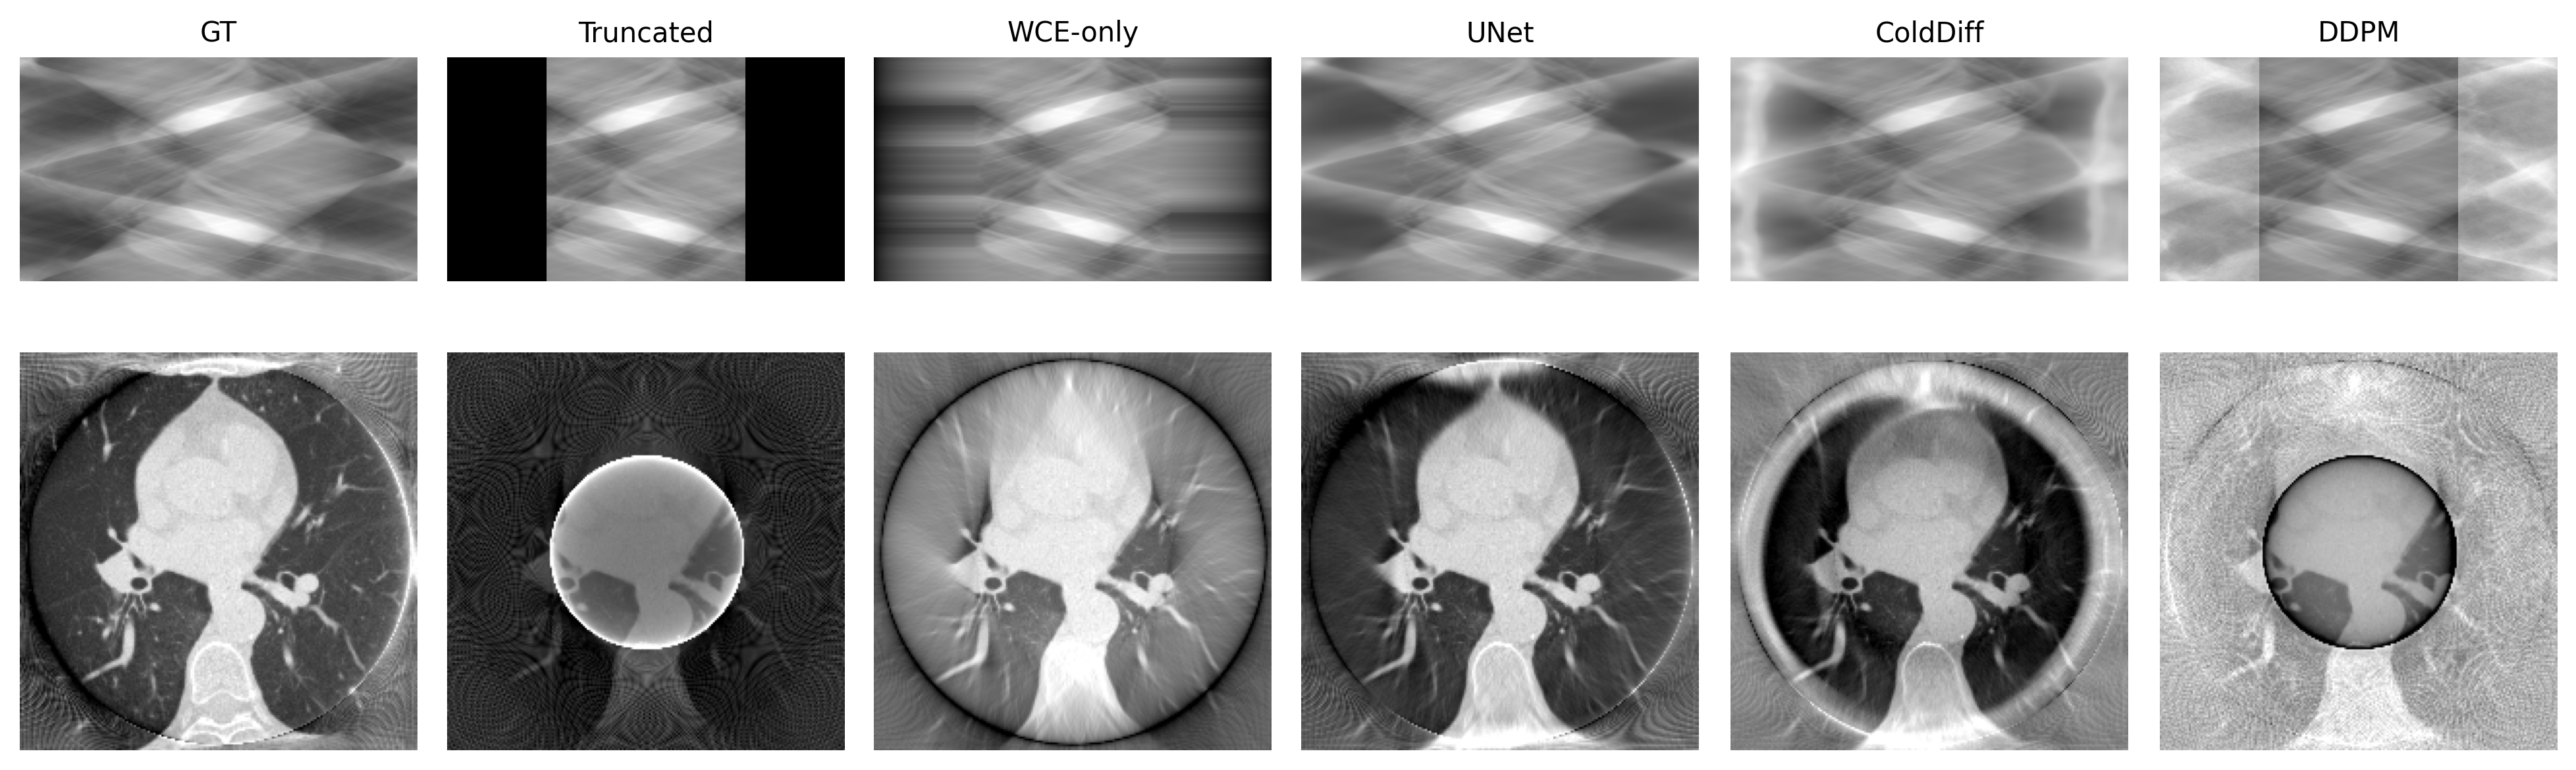
\includegraphics[width=\textwidth]{figures/baseline_merged_lidc0450.png}
\caption{Qualitative baseline comparison on a representative sample from the LIDC-IDRI dataset. Columns: GT, Truncated, WCE-only, UNet, ColdDiff, DDPM. Top row: sinogram domain. Bottom row: FDK-like reconstruction domain.}
\label{fig:baseline_qualitative_lidc0450}
\end{figure}

To complement the LIDC example, Figure~\ref{fig:baseline_qualitative_ctorg38} shows a representative CT-ORG case under the same truncation setting. The same ordering is observed: WCE-only softens hard truncation boundaries but retains reconstruction artifacts, U-Net is closest to GT in global structure and local contrast, Cold Diffusion yields visibly cleaner recovery than DDPM, and DDPM remains the noisiest among learned methods.

\begin{figure}[H]
\centering
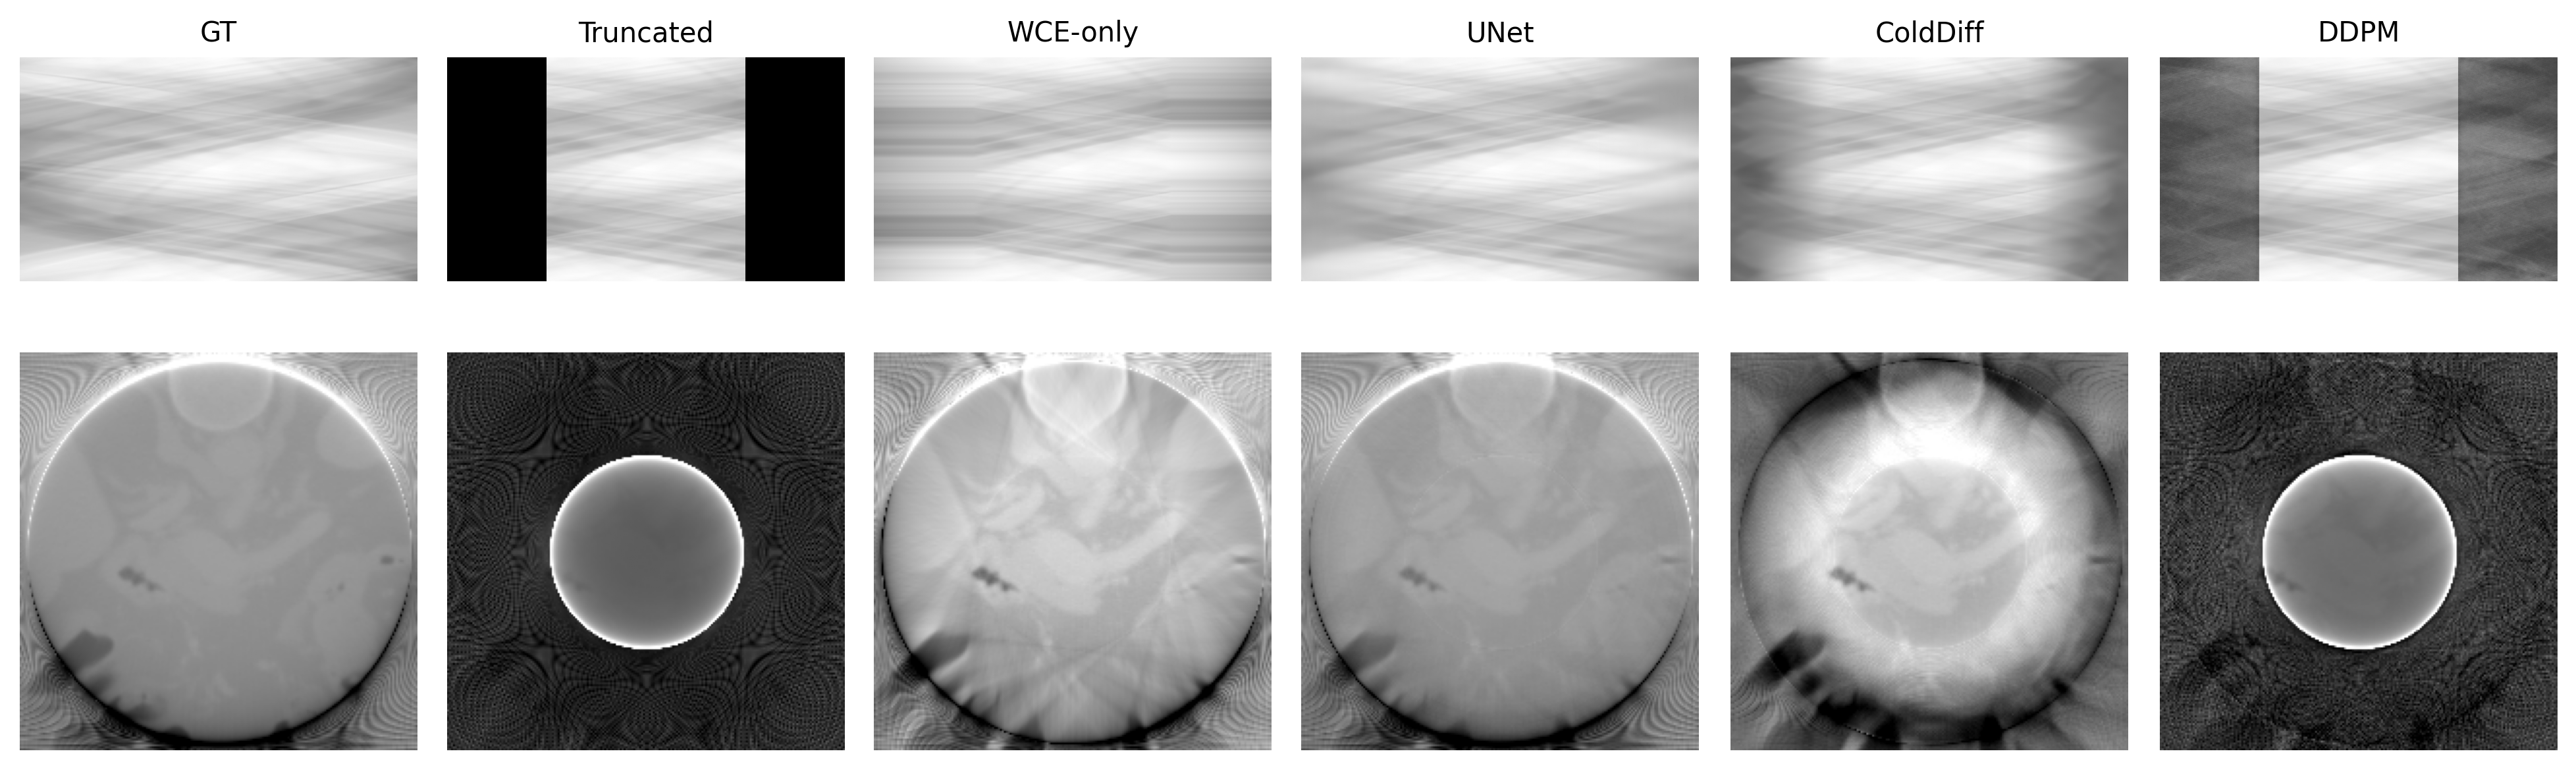
\includegraphics[width=\textwidth]{figures/baseline_merged_ctorg38.png}
\caption{Qualitative baseline comparison on a representative sample from the CT-ORG dataset (\(k_c=320\)). Columns: GT, Truncated, WCE-only, UNet, ColdDiff, DDPM. Top row: sinogram domain. Bottom row: FDK-like reconstruction domain.}
\label{fig:baseline_qualitative_ctorg38}
\end{figure}

\subsection{Comparison Dimensions}

The baseline analysis covers sinogram-domain PSNR, SSIM, and MAE, reconstruction-domain PSNR and SSIM after FDK-like reconstruction, and per-dataset behavior on CT-ORG and LIDC-IDRI.

\section{Training Dynamics and Convergence}

\subsection{Training Monitoring Protocol}

Model training is monitored through complementary signals to ensure proper convergence and identify potential issues early. The L1 loss is tracked throughout training and checkpoints are saved regularly. Model selection follows the fixed-step training schedule.

\subsection{Observed Training Characteristics}

Training logs show stable optimization behavior across the fixed-step trajectory, with consistent checkpoint progression.

For the timestep-related Cold Diffusion runs, this fixed-step trajectory is instantiated by the paired \(T=50\) and \(T=150\) configurations. Both settings are trained to 150,000 steps with the same checkpoint interval and evaluated through the same batched seed pipeline, so the timestep factor is controlled within one reproducible training and evaluation path.

\subsection{Timestep Result}

We also report a timestep comparison. This run uses the same seed set \(\{42,52,62,72\}\), fixed truncation ratio 0.25 for evaluation, and the same aggregation procedure over seed outputs. The paired timestep models are trained at truncation ratio 0.75 and evaluated at 0.25 under a matched test protocol to isolate timestep effects.

Table~\ref{tab:Timestep_summary} summarizes the 4-seed aggregate. In reconstruction space, \(T=150\) is clearly stronger than \(T=50\) (FBP PSNR \(44.52\pm0.77\) dB vs.\ \(37.75\pm1.06\) dB; FBP SSIM \(0.936\pm0.010\) vs.\ \(0.862\pm0.024\)). In sinogram space, \(T=50\) attains lower MAE/RMSE and higher PSNR than \(T=150\), while \(T=150\) yields higher ROI-SSIM in the truncated band. This mismatch indicates that lower pixel-wise sinogram error does not always translate into better post-FBP image quality under the same truncation setting.
To avoid misinterpretation, this timestep study is a controlled comparison within the same training chain: all non-timestep design factors are kept matched inside that chain, and the conclusions are limited to relative \(T=50\) vs.\ \(T=150\) behavior under the same protocol. Accordingly, the timestep numbers are not interpreted as a direct replacement for, or direct one-to-one comparison against, the baseline table above.

\begin{table}[htbp]
\centering
\caption{Fast timestep aggregate (4 seeds). Values are mean \(\pm\) std over seeds.}
\label{tab:Timestep_summary}
\begin{tabular}{lcccc}
\toprule
\textbf{Method} & \textbf{FBP PSNR} & \textbf{FBP SSIM} & \textbf{Sino MAE} & \textbf{Sino PSNR} \\
\midrule
Truncated & \(29.39 \pm 0.99\) & \(0.525 \pm 0.031\) & \(50.67 \pm 3.74\) & \(10.72 \pm 0.44\) \\
WCE-only & \(42.23 \pm 0.65\) & \(0.888 \pm 0.016\) & \(5.60 \pm 0.58\) & \(27.73 \pm 1.07\) \\
Cold Diffusion (\(T=50\)) & \(37.75 \pm 1.06\) & \(0.862 \pm 0.024\) & \(2.97 \pm 0.12\) & \(30.49 \pm 1.02\) \\
Cold Diffusion (\(T=150\)) & \(44.52 \pm 0.77\) & \(0.936 \pm 0.010\) & \(5.83 \pm 0.32\) & \(28.01 \pm 0.88\) \\
\bottomrule
\end{tabular}
\end{table}

\begin{figure}[H]
\centering
\begin{minipage}{0.48\textwidth}
\centering
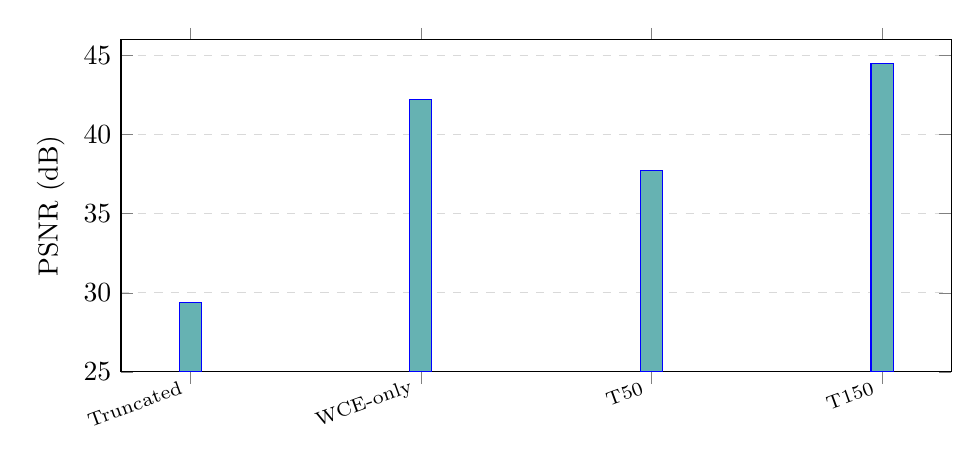
\begin{tikzpicture}
\begin{axis}[
    ybar,
    bar width=8pt,
    width=\textwidth,
    height=5.8cm,
    ymin=25,
    ymax=46,
    ylabel={PSNR (dB)},
    symbolic x coords={Truncated,WCE-only,T50,T150},
    xtick=data,
    xticklabel style={font=\scriptsize, rotate=20, anchor=east},
    ymajorgrids=true,
    grid style={dashed,gray!30}
]
\addplot+[fill=teal!60] coordinates {(Truncated,29.39) (WCE-only,42.23) (T50,37.75) (T150,44.52)};
\end{axis}
\end{tikzpicture}
\end{minipage}
\hfill
\begin{minipage}{0.48\textwidth}
\centering
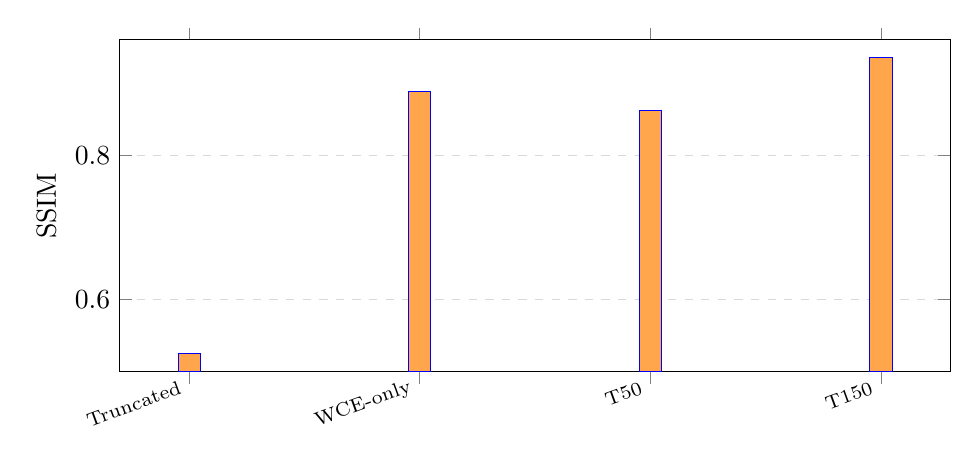
\begin{tikzpicture}
\begin{axis}[
    ybar,
    bar width=8pt,
    width=\textwidth,
    height=5.8cm,
    ymin=0.50,
    ymax=0.96,
    ylabel={SSIM},
    symbolic x coords={Truncated,WCE-only,T50,T150},
    xtick=data,
    xticklabel style={font=\scriptsize, rotate=20, anchor=east},
    ymajorgrids=true,
    grid style={dashed,gray!30}
]
\addplot+[fill=orange!70] coordinates {(Truncated,0.525) (WCE-only,0.888) (T50,0.862) (T150,0.936)};
\end{axis}
\end{tikzpicture}
\end{minipage}
\caption{Fast reconstruction-domain comparison. \(T=150\) provides the best FBP-domain quality in both PSNR and SSIM.}
\label{fig:exp3_fast_fbp}
\end{figure}

\begin{figure}[H]
\centering
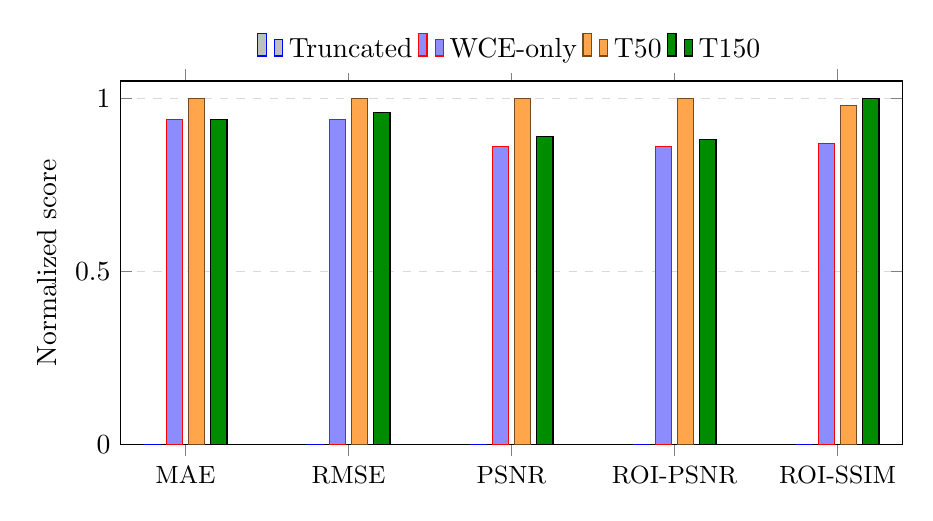
\begin{tikzpicture}
\begin{axis}[
    ybar,
    bar width=6pt,
    width=0.95\textwidth,
    height=6.2cm,
    ymin=0,
    ymax=1.05,
    ylabel={Normalized score},
    symbolic x coords={MAE,RMSE,PSNR,ROI-PSNR,ROI-SSIM},
    xtick=data,
    xticklabel style={font=\small},
    legend style={at={(0.5,1.02)}, anchor=south, legend columns=4, draw=none},
    ymajorgrids=true,
    grid style={dashed,gray!30}
]
\addplot+[fill=gray!50] coordinates {(MAE,0.00) (RMSE,0.00) (PSNR,0.00) (ROI-PSNR,0.00) (ROI-SSIM,0.00)};
\addplot+[fill=blue!45] coordinates {(MAE,0.94) (RMSE,0.94) (PSNR,0.86) (ROI-PSNR,0.86) (ROI-SSIM,0.87)};
\addplot+[fill=orange!70] coordinates {(MAE,1.00) (RMSE,1.00) (PSNR,1.00) (ROI-PSNR,1.00) (ROI-SSIM,0.98)};
\addplot+[fill=green!55!black] coordinates {(MAE,0.94) (RMSE,0.96) (PSNR,0.89) (ROI-PSNR,0.88) (ROI-SSIM,1.00)};
\legend{Truncated,WCE-only,T50,T150}
\end{axis}
\end{tikzpicture}
\caption{Direction-aware normalized sinogram metrics for fast results. Lower-is-better metrics (MAE, RMSE) are inverted before normalization. This view highlights that \(T=50\) dominates in several sinogram error metrics, while \(T=150\) is strongest in ROI-SSIM.}
\label{fig:exp3_fast_sino_norm}
\end{figure}

\section{Visualization and Qualitative Analysis}

\subsection{Visual Comparison Framework}

Qualitative assessment uses sinogram comparisons (truncated input vs.\ prediction vs.\ ground truth) and corresponding cone-beam filtered backprojection reconstructions. The objective is to connect numerical trends to visually interpretable failure modes, especially boundary discontinuities and streak artifacts that can persist even when PSNR improves.

\subsection{Case Selection Criteria}

Visual examples are selected according to a stratified sampling strategy to represent the full performance spectrum. Typical cases with median reconstruction error illustrate expected behavior on most inputs. Best cases with minimal error demonstrate the achievable ceiling under favorable conditions. Challenging cases expose failure modes and guide hypotheses about truncation boundaries, local contrast, and anatomy-specific ambiguity. Anatomical diversity is preserved by including both abdominal (CT-ORG) and thoracic (LIDC-IDRI) examples to assess cross-region robustness.

\section{Summary of Evaluation Framework}

This chapter reports the evaluation framework and the executed results from the 4-seed baseline aggregation, where U-Net inpainting performs best, Cold Diffusion outperforms DDPM, and DDPM remains below WCE-only under the tested setup.

\section{Current Interpretation}

The baseline comparison consistently shows that U-Net inpainting is strongest, Cold Diffusion is better than DDPM, and DDPM remains below the WCE-only reference in the present setup. The cross-dataset analysis on CT-ORG and LIDC-IDRI shows the same relative ordering, which suggests that the current ranking is not driven by a single anatomy source.
